\documentclass[paper=a4,11pt,titlepage,twoside=true,headings=normal,numbers=noenddot,captions=tableabove,listof=totoc,index=totoc,bibliography=totoc,german]{scrreprt}
%\usepackage{amsmath} % abgesetzte Formeln zentriert in der Zeile
%\usepackage[fleqn,intlimits]{amsmath} % [fleqn] abgesetzte Formeln mit festem Abstand zum linken Rand
\usepackage[reqno,intlimits]{amsmath} % [reqno] um die gleichungsnummerierung rechts zu haben
% intlimits: Grenzen für Integrale unterhalb und oberhalb des Zeichens
\usepackage{amssymb}
\usepackage{array}
\usepackage[ngerman]{babel}
\usepackage[ngerman]{varioref}
\usepackage[T1]{fontenc} 
\usepackage[utf8]{inputenc}
%---------------------------
\usepackage{booktabs}
\usepackage{calc}
\usepackage{cancel}
\usepackage[labelfont={footnotesize,sf,bf},textfont={footnotesize,sf}]{caption} %Format (Textgröße, Textform) für Bildtext 
%normalsize
%scriptsize
% sc --> smallcaps
% bf --> bold face
% sf --> sans serif
%\usepackage{cite} %inkompatibel mit biblatex
\usepackage[table]{xcolor}
%\usepackage{colortbl}
\usepackage[right]{eurosym}
%\usepackage{caption2} %nicht zusammen mit sidecap
%\usepackage{exscale}
\usepackage{ellipsis}
\usepackage{graphicx}
\usepackage{float}
%\usepackage{floatflt}
%----------------------------------------
\usepackage{gensymb} %-----------
%\usepackage{helvet}
\usepackage{csquotes}
\usepackage{listings}
\usepackage{longtable}
\usepackage{lastpage}  %----------
\usepackage{lscape}
\usepackage{lmodern}  %-- Silbentrennung
%\usepackage{mathpazo} % andere mathematische Symbol
\usepackage{makeidx}
%\usepackage{minitoc}
\usepackage{multirow}
\usepackage{multicol}
%\usepackage[intoc]{nomencl}   % zwei Spalten beim Formelzeichenverzeichnis
\usepackage[german,intoc]{nomentbl} %vier Spalten bei Formelzeichenverzeichnis
\usepackage{nicefrac} %----
%\usepackage{picins} %----------
\usepackage{paralist} %--------
\usepackage{parallel}  %----------
\usepackage{pdfpages} %-------
% Define user colors using the RGB model
%\usepackage{colortbl}
%\definecolor{dunkelgrau}{rgb}{0.8,0.8,0.8}
%\definecolor{hellgrau}{rgb}{0.95,0.95,0.95}
%\usepackage{pgfplots}
\usepackage[figuresright]{rotating} 
\usepackage{scrlayer-scrpage}
%\usepackage[innercaption]{sidecap} %Beschriftung neben Bild, Tabelle, Mittelbach S333 %----------
% \usepackage{sistyle}
% \usepackage[locale=DE]{siunitx} %nicht zusammen mit sistyle %---------
\usepackage[locale=DE,parse-numbers=false]{siunitx} %nicht zusammen mit sistyle %---------
\sisetup{
	per-mode=fraction,
	% quotient-mode=fraction,
	fraction-function=\tfrac
}
% \usepackage[locale=DE,parse-numbers=false]{siunitx} %nicht zusammen mit sistyle %---------
\usepackage[font={scriptsize,sl},captionskip=3pt]{subfig} % für die Unterbilder %---------
\usepackage{shortvrb}
\usepackage{tablefootnote}
\usepackage{tabularx}
\usepackage{tabulary}
\usepackage{textcomp}
\usepackage{tocbasic}
%\usepackage{tikz}
\usepackage{times} 
\usepackage{units} %----------
\usepackage{url}
\usepackage{wrapfig} %----------
\usepackage{xr-hyper}
\usepackage{arydshln} %für \hdashline[5pt/2pt] % muss am Ende stehen, sonst gibt es Probleme mit xcolor
\usepackage{hyperref} % muss am Schluss stehen
\hypersetup{linkcolor={0 1 1}, linkbordercolor={1 1 1}, citebordercolor={1 1 1}} % setzt Linkboxen auf Farbe "`weiß"'
%\usepackage{bm}
%\usepackage[toc,symbols]{glossaries} %---------- muss nach hyperref stehen
\usepackage[nonumberlist, acronym, toc, section]{glossaries} % muss nach hypersetup stehen
%----------------
%\usepackage{romannum} % Seitenzahlen in römischen Ziffern
%\usepackage{adjustbox}
\usepackage{scrhack}
\usepackage[style=numeric, citestyle=numeric, backend=biber]{biblatex}
\usepackage{cleveref} % löscht labels!!!!!!!!!!
%-------------------------
 %\renewcommand{\captionlabelfont}{\sffamily} %für "Abbildung" und "Tabelle"
 %\renewcommand{\captionfont}{\sffamily\small} %für den Text der Bildunterschriften
%  \renewcommand{\captionlabelfont}{\sffamily} 
%  \renewcommand{\captionfont}{\sffamily} %\renewcommand{\normalfont}{\sffamily} %für die Überschriften
% Fettdruck der Bezeichnung Abbildung, Tabelle
%\renewcommand{\captionlabelfont}{\bfseries}
%---------------------------------------------
%------------------ Schrifttyp in der Kopf- und Fusszeilen
\setkomafont{pageheadfoot}{\footnotesize\sffamily}
%---------------------------------------------------
%Ändern der Abbildung- und Tabellenbezeichnung (Niedermair S.157)
%_____________________________________________
\addto\captionsngerman{\renewcommand\figurename{Abb.}}
\addto\captionsngerman{\renewcommand\tablename{Tab.}}
\renewcommand\listfigurename{Abbildungen}
%_______________________________
%Betrag eines Wertes
\newcommand{\abs}[1]{\lvert #1 \rvert} 
%---------------------------------------------
\newcommand{\absatz}[1]{\textbf{\textsc{#1}}} %siehe Mittelbach S. 876ff
%----------------------------
%\newcommand{\absatz}{\par \medskip}
%______________________________
%\newcommand{\anhang}[1]{Anhang \ref{#1}, Seite \pageref{#1}}
\newcommand{\anhang}[1]{Anhang \vref{#1}}
%________________________________
\newcommand{\aufgabe}{\stepcounter{plus} Aufgabe \arabic{plus}}
%______________________________________
%compactitem
\newcommand{\bci}{\begin{compactitem}}
\newcommand{\eci}{\end{compactitem}}
%______________________________________
%
\newcommand{\bi}{\begin{itemize}}
\newcommand{\ei}{\end{itemize}}
%______________________________________
%compactenumerate
\newcommand{\bce}{\begin{compactenum}}
\newcommand{\ece}{\end{compactenum}}
%_____________________________________
%begin equation
\newcommand{\be}{\begin{equation}}
\newcommand{\ee}{\end{equation}}
%_____________________________________
%begin equation ohne Formelnummer
\newcommand{\ben}{\begin{equation*}}
\newcommand{\een}{\end{equation*}}
%_____________________________________
%begin align ohne Formelnummer
\newcommand{\ban}{\begin{align*}}
\newcommand{\ean}{\end{align*}}
%_____________________________________
%begin align
\newcommand{\ba}{\begin{align} }
\newcommand{\ea}{\end{align}}
%_____________________________________
%minpage
\newcommand{\bmp}{\begin{minipage}[t]{.47\linewidth}}
\newcommand{\emp}{\end{minipage}}
%_____________________________
%  dB
\newcommand{\db}{dB}
%  dB(A)
\newcommand{\dba}{ dB(A) }
%  dB(A) für Satzende
\newcommand{\dbap}{ dB(A)}
%_________________________________
\newcommand{\bzw}{bzw.\,}
%_______________________________
\newcommand{\dif}{\mathrm{d}}
%________________________________
% neuer Zähler
\newcounter{plus}
\setcounter{plus}{0}
%______________________________
%Für das Formelverzeichnis _____________________ Formelverzeichis ____
% Befehl umbenennen in fz
\let\fz\nomenclature
% Deutsche Überschrift
\renewcommand{\nomname}{Formelzeichen}
% Punkte zw. Abkürzung und Erklärung
\setlength{\nomlabelwidth}{.20\hsize}
\renewcommand{\nomlabel}[1]{#1 \dotfill}
% Zeilenabstände verkleinern
\setlength{\nomitemsep}{-\parsep}
%_____________________________
\newcommand{\bild}[1]{Abb. \vref{#1}}
\newcommand{\sbild}[1]{siehe Abb. \vref{#1}}
\newcommand{\bilder}[2]{Abb. \vrefrange{#1}{#2}}
\newcommand{\bildseite}[1]{Abb. \vref{#1}} % erzeugt "`Abb. nn auf Seite nn
\newcommand{\tabelle}[1]{Tab. \vref{#1}}
\newcommand{\tabellenseite}[1]{Tab. \vref{#1}} % erzeugt "`Tab. nn auf Seite nn
% für \vref ist usepackage[german]{varioref} einzufügen
%_-------------------------------- Freiraum
\newcommand{\freiraum}[1]{\begin{figure}[H]\vspace{#1\textheight}\end{figure}}
%_____________________________
% Gleichung
\newcommand{\gl}[1]{Gl.\,(\ref{#1})}
\newcommand{\sgl}[1]{siehe Gl.\,(\ref{#1})}
\newcommand{\glbereich}[2]{Gl. \vrefrange[]{#1}{#2}}
%_____________________________
% Grad Celsius
\newcommand{\grad}{\,\degC}
\newcommand{\gradC}{\,\degree}
%______________________________________
% Großbuchstaben als Indizes kleiner schreiben; spezielle im Mathemodus
\newcommand{\klein}[1]{\scriptscriptstyle{#1}}% Fettdruck der Bezeichnung 
%______________________________
%% Kasten
\newcommand{\kasten}{\fbox{\rule{0.0pt}{10pt}{{ } } }}
%______________________________
%\newcommand{\kapitel}[1]{Kapitel \ref{#1}, Seite \pageref{#1}}
\newcommand{\kapitel}[1]{Kapitel \vref{#1}}
%_____________________________
%  LAeq für den äquivalenten Dauerschallpegel
\newcommand{\laeq}{ $L_{Aeq}$ }
%  LAeq für den äquivalenten Dauerschallpegel am Satzende
\newcommand{\laeqp}{ $L_{Aeq}$}
%_________________________________
%   Linie zeichnen
\newcommand{\linie}{\rule{0.5\textwidth}{0.1pt}}
%---------------------- LaTeX
\newcommand{\lt}{\LaTeX\,\,}
%----------------------------
\newcommand{\nl}{\newline}
%__________________________________
%  multicolumn für Tabellen
\newcommand{\mc}{\multicolumn}
%% \mc{1}{c}{Text}
%_________________________________
%    Parallel
\newcommand{\pl}[1]{\ParallelLText{#1}}
\newcommand{\pr}[1]{\ParallelRText{#1}}
\newcommand{\pp}{\ParallelPar}
%------------ rot unterstrichen
\newcommand{\rotunterstrichen}[1]{\textcolor{red}{\underline{\textcolor{black}{#1}}}}
%________________ Realteil
\newcommand{\real}[1]{\text{Re}\left\{#1\right\}}
%________________________________--
\newcommand{\seite}[1]{Seite \pageref{#1}}
\newcommand{\seiten}[2]{\vpagerefrange{#1}{#2}}
%----------------------------
%        TEXT Rot
\newcommand{\textrot}[1]{\textcolor{red}{#1}}
%______________________________
%Abkürzung für \multicolumn
\newcommand{\tab}[2]{\multicolumn{1}{#1}{#2}}
%_____________________________________
% doppelt unterstreichen
\newcommand{\unterstreichen}[1]{\underline{\underline{#1}}}
% einfach unterstreichen
\newcommand{\ul}[1]{\underline{#1}}
%______________________________
%kurze Verbatimausgabe
%\MakeShortVerb{\|} %mittelbach S.160 mit \usepackage{shortvrb}
%_______________________________________
% vspace
\newcommand{\vsf}{\vspace{5pt}}
%_________________________________
\newcommand{\zb}{z.B.\,}
\newcommand{\idr}{i.d.R.\,}
%_______________________________
% Zähler-einfach
\newcounter{req}
\newcommand{\zaehler}[1]{\refstepcounter{req}{#1} \thereq}
%% Beispielaufzählung \zaehler{Beispiel}\\
%_____________________________________
 \setlength{\voffset}{-2.532 cm}
 \setlength{\hoffset}{-1.57 cm}
% \setlength{\topmargin}{2.0 cm} \setlength{\topskip}{0.1 cm}
 \setlength{\topmargin}{1.5 cm}
 \setlength{\topskip}{0.1 cm}
 \setlength{\evensidemargin}{1.5 cm}
 \setlength{\oddsidemargin}{1.5 cm}
 \setlength{\textwidth}{16.5 cm}
 \setlength{\footskip}{40pt}
 \setlength{\textheight}{24.5cm}
% \setlength{\textheight}{23.5 cm}
 \setcounter{page}{1}
 \setlength{\parindent}{0cm}
 \setlength{\headsep}{20pt}
%----------------------------------------------------------------------
% Linien in der Kopf- und Fußzeile
%\renewcommand{\headrulewidth}{0.0pt}   %Linie in der Kopfzeile mit 0.0pt keine Linie
%%\renewcommand{\footrulewidth}{0.0pt}   %Linie in der Fußzeile mit 0.0 pt keine Linie
%\renewcommand{\headrulewidth}{0.2pt}   %Linie in der Kopfzeile mit 0.0pt keine Linie
%\renewcommand{\footrulewidth}{0.2pt}   %Linie in der Fußzeile mit 0.0 pt keine Linie
%------------------------------------------------------------------------
%\renewcommand{\normalfont}{\sffamily} %für die Überschriften
%\renewcommand{\chaptermark}[1]{\markboth{\chaptername\ \thechapter #1}{}}
%\renewcommand{\sectionmark}[1]{\markright{\thesection\ #1}}
% \rfoot{\leftmark\\\rightmark}

%Definitionen für Kopfzeile
% bei documentclass {report} hat der Eintrag für die [gerade Seite] keine Wirkung
%-------------------------------------------------------------
%%
%Einstellungen für Kopf- und Fusszeilen mit dem KOMA-Skript und \usepackage{scrpage2}
\pagestyle{scrheadings}
%\pagestyle{scrplain}
% le --> links, gerade Seite
% ce --> mittig, gerade Seite
% re --> rechts, gerade Seite
% lo --> links, ungerade Seite
% co --> mittig, ungerade Seite
% ro --> rechts, ungerade Seite
%---------------------------------------------
% Löschen aller Einträge
%\clearscrheadings
% \automark[section]{subsection}
% \pagemark --> Seitenzahl
% \automark --> Kapitelüberschriften
% \leftmark --> ??
% \rightmark --> ??
%::::::::::::::::::::::::::::::::::: Kopfzeile
% Kopfzeile gerade Seite
\automark[chapter]{chapter}
\lehead[]{\titelkopfzeilelinkseven}
\cehead[]{\titelkopfzeilemitteeven}
\rehead[]{\titelkopfzeilerechtseven}
% Kopfzeile ungerade Seite
\lohead[]{\titelkopfzeilelinksodd}
\cohead[]{\titelkopfzeilemitteodd}
\rohead[]{\titelkopfzeilerechtsodd}
% Linie in der Kopfzeile
%\setheadtopline{0.2pt} % obere Linie in der Kopfzeile; nur bei scrartcl
\setheadsepline{0.4pt} % untere Linie in der Kopfzeile; nur bei scrartcl
% Linie in der Fusszeile
%::::::::::::::::::::::::::::::::::: Fußzeile
% Fusszeile gerade Seite[plain-style]{scrheadings-style}
\lefoot[]{\titelfusszeilelinkseven} 
\cefoot[]{\titelfusszeilemitteeven}
\refoot[]{\titelfusszeilerechtseven}
% Fusszeile ungerade Seite
\lofoot[]{\titelfusszeilelinksodd}
\cofoot[]{\titelfusszeilemitteodd}
\rofoot[]{\titelfusszeilerechtsodd}
%\rofoot[\thepage ]{\thepage}
%\setfoottopline{0.2pt} % obere Linie in der Kopfzeile; nur bei scrartcl
\setfootsepline{0.4pt} % untere Linie in der Kopfzeile; nur bei scrartcl

% le --> links, gerade Seite
% ce --> mittig, gerade Seite
% re --> rechts, gerade Seite
% lo --> links, ungerade Seite
% co --> mittig, ungerade Seite
% ro --> rechts, ungerade Seite
% even --> gerade Seite
% odd --> ungerade Seite
%----------------------------------------- Kopfzeilentext
 \newcommand{\titelkopfzeilemitteeven}{}
 \newcommand{\titelkopfzeilemitteodd}{}
 \newcommand{\titelkopfzeilelinkseven}{Hochschule RheinMain}
 \newcommand{\titelkopfzeilelinksodd}{}
 \newcommand{\titelkopfzeilerechtseven}{}
 \newcommand{\titelkopfzeilerechtsodd}{Hochschule RheinMain}
 %----------------------------------------- Fußzeilentext
 \newcommand{\titelfusszeilemitteeven}{}
 \newcommand{\titelfusszeilemitteodd}{}
 \newcommand{\titelfusszeilerechtseven}{Studienbereich Angewandte Physik \& Medizintechnik}
 \newcommand{\titelfusszeilerechtsodd}{\thepage \hspace{0.5mm} von \pageref{LastPage}}
 \newcommand{\titelfusszeilelinkseven}{\thepage \hspace{0.5mm} von \pageref{LastPage}}
 \newcommand{\titelfusszeilelinksodd}{Studienbereich Angewandte Physik \& Medizintechnik}
\newcommand{\titelLV}{Physikalisches Praktikum 2}
%---------------------------- VARIABLEN festlegen ------------------
%----------- Pro Versuch zu ändernde Angaben -----------------------
% \newcommand{\versuch}{3} % Versuchsnummer einfügen
\newcommand{\untertitelb}{Hall-Effekt} % Titel des Versuchs einfügen
\newcommand{\datumLV}{23.10.2020} % Datum einfügen
\newcommand{\deadline}{14.11.2020} % Datum einfügen
%----------- TITEL
\newcommand{\untertitela}{Versuch P2-6}
% -------- Student 1
\newcommand{\nameA}{Herr Cihan Ünlü}
% --------- Student 2
\newcommand{\nameB}{Herr Dennis Hunter}
% --------- Student 3, falls vorhanden
\newcommand{\nameC}{Herr Student drei}
%::::::::::::::::::::::::::::::::::
%\input{chapters/glossar}
\addbibresource{quellen.bib}
\begin{document}
%-----------------------------------------------------------------
\begin{titlepage} 
	\newcommand{\HRule}{\rule{\linewidth}{0.5mm}} 	
	\centering
	\textsc{\Large Hochschule RheinMain \\
		
\includegraphics[width=0.15\textwidth]{logo-hsrm}\\[1cm]}
%	\textsc{\Large Hochschule RheinMain}\\[1cm]
	\textsc{\LARGE \titelLV}\\[0.5cm]
		\HRule\\[0.4cm]
	{\huge\bfseries \untertitela}\\[0.4cm] % Title des Dokuments
	{\huge\bfseries \untertitelb}\\[0.4cm] % Title des Dokuments
		\HRule\\[1.5cm]
%-------------------
%\begin{flushleft}
	\begin{minipage}{0.4\textwidth}
%	\begin{flushleft}
%\centering
		\large
		\textit{\underline{Autoren}}\\[0.5cm]
		\textsc{\nameA}\\[0.5cm]
		\textsc{\nameB}\\[0.5cm]
		%\textsc{\nameC}\\[0.5cm] 
%	\end{flushleft}
\end{minipage}
%------------------------------------
\vfill\vfill\vfill 
\textsc{\Large Fachbereich Ingenieurwissenschaften}\\[0.5cm]
\textsc{\large Studienbereich Angewandte Physik \& Medizintechnik}\\[0.5cm] 
\vfill	
Datum des Versuchs:\hspace{0.4cm} {\large\datumLV}\\
Abgabedatum:\hspace{0.4cm} {\large\deadline} 
\end{titlepage}

%-----------------------------------------------------
\tableofcontents
\newpage
%--------------------
\chapter{Einleitung}
%Ziel des Versuchs.
Im Laufe dieses Versuchs kommen sowohl Größen aus der Magneto-, als auch der Elektrostatik zur Anwendung. Im Folgenden
sollen wichtige Messtechnische Größen durch relevante Gleichungen in Zusammenhang gebracht werden.
\section{Grundlagen}
    %Phys. und Messtechn. Grundlagen
    Im Folgenden soll sich zur Bezeichnung der Dimensionen des \textsc{Hall}-Plättchens in \cref{fig:hall_dim} gezeigte
    Konvention angewandt werden.
    \begin{figure}[H]
        \centering
        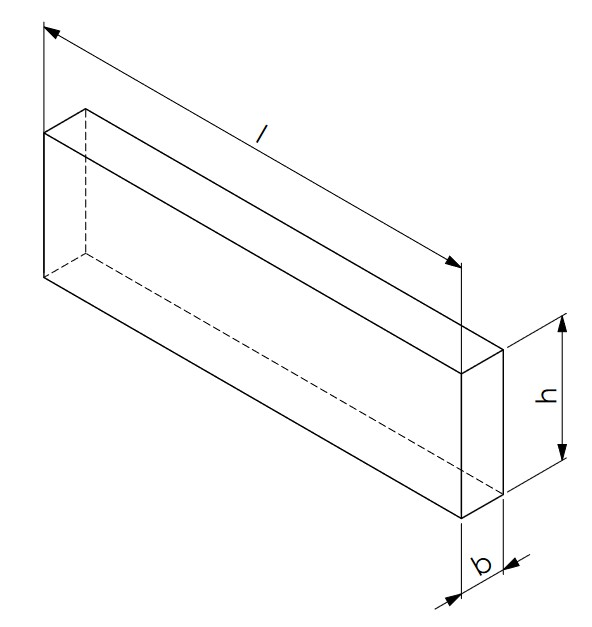
\includegraphics[width=.6\textwidth]{CAD/hall_dim.jpg}%
        \caption[Konvention der Längenbezeichnungen]{In diesem Dokument angewandte Längenbezeichnungen eines \textsc{Hall}-Plättchens mit \(h\) für
        \textit{Höhe}, \(b\) für \textit{Breite} und \(l\) für \text{Länge}.}%
        \label{fig:hall_dim}
    \end{figure}
    Damit für den spezifischen Widerstand eines Materials:
    \begin{equation}
        R = \rho \cdot \frac{l}{b h} \quad \Leftrightarrow \quad \rho = R \cdot \frac{b h}{l}%
        \label{eq:spezR}
    \end{equation}
    \subsection{\textsc{Hall}-Spannung}
        Befindet sich ein Stromdurchflossener Leiter der Breite \(b\), Höhe \(h\) und Länge \(l\) innerhalb eines externen Magnetfeldes
        \( \vec{B} \) erfahren bewegte Ladungsträger eine Kraft \(\vec{F_L}\), die orthogonal zum Magnetfeld und ihrer Bewegungsrichtung
        \( \vec{v} \) (\cref{eq:lorentz}) gerichtet ist.
        %
        \begin{equation}
            \vec{F_L} = q \cdot (\vec{v_D} \times \vec{B})%
            \label{eq:lorentz}
        \end{equation}
        %
        Die Ladungsträger können nicht über die Leiteroberfläche hinaus ausweichen und es kommt zu einer Ladungsträgerverdichtung
        auf einer Seite des Leiters und entsprechend zu einer betragsgleichen Verknappung auf der gegenüberliegenden Seite. Bei
        einer Trennung von Ladungsträgern bildet sich ein elektrisches Feld aus welches wiederum nach \cref{eq:elektrische_kraft}
        der Lorentzkraft entgegen wirkt.
        %
        \begin{equation}
            \vec{F_E} = q \vec{E}
            \label{eq:elektrische_kraft}
        \end{equation}
        %
        Im statischen Fall kommt es zu einem Gleichgewicht zwischen der elektrischen Feldkraft \(\vec{F_E}\) und der Lorentzkraft
        \(\vec{F_L}\) nach
        \begin{align}
            \vec{F_E} &= \vec{F_L} \nonumber\\
            q \cdot \vec{E} &= q \cdot (\vec{v_D} \times \vec{B}) \nonumber\\
            \frac{\vec{U_H}}{h} &= \vec{v_D} \times \vec{B} \nonumber\\
            \vec{U_H} &= h \cdot (\vec{v_D} \times \vec{B})
            \label{eq:UH1}
        \end{align}
        bzw. für den Fall, dass alle drei Vektorielle Größen jeweils orthogonal zueinander stehen:
        \begin{equation}
            U_H = h v_D B
            \label{eq:UH1ez}
        \end{equation}

        Da die Stromdichte durch die Probe mit der durchflossenen Fläche durch \(I_p = b\cdot h \cdot j\) gerade den Probenstrom ergibt
        und mit der Driftgeschwindigkeit der Ladungsträger als \(v_D=j \cdot (q\cdot n_q)\) lässt sich \cref{eq:UH1ez} überführen zu
        \begin{align}
            U_H = \frac{I_p}{b j} \cdot B \cdot \frac{j}{q n_q} = \frac{B \cdot I_p}{q n_q b}
            \label{eq:UH2}
        \end{align}
    \subsection{Magnetischer Kreis}
        %
        Das magnetische Durchflutungsgesetz bildet einen Zusammenhang zwischen der magnetischen Durchflutung \(\Theta\) und
        dem durch sie eingeschlossenen Strom \(I\) nach \cite{Halliday.2005}
        \begin{equation}
            \Theta = \oint \vec{H} \bullet d\vec{s} = I
        \end{equation}
        Im Falle einer Spule mit Eisenkern lässt sich dieser Zusammenhang vereinfacht darstellen durch
        \begin{equation}
            \Theta = N \cdot I
            \label{eq:NI}
        \end{equation}
        wobei \(N\) die Windungszahl der Spule und \(I\) der in den Windungen fließende Strom ist.

        In Analogie zum ohm'schen Gesetz gilt weiter
        \begin{equation}
            \Theta = \Phi \sum\limits_{}^{i} R_{m,i}
        \end{equation}
        mit
        \begin{equation}
            R_{m,i} = \frac{s_i}{\mu_0\mu_{r,i} A}
            \label{eq:Rm}
        \end{equation}
        Hier ist \(\Phi\) der magn. Fluss in der Einheit \(\SI{}{Wb}\), \(\mu_0\) die magn. Feldkonstante (auch Permeabilität des
        Vakuums) mit \(\approx 4\pi \cdot \SI{10^{-7}}{\newton\per\ampere\squared}\), \(\mu_r\) die (einheitenlose) materialabhängige relative
        Permeabilität und \(s\) und \(A\) die durchflutete Strecke respektive Fläche in den Einheiten \(\si{m}\) und \(\si{m\squared}\).
    %     %\section{Gleichungen und Herleitungen}
    %     %Herleitung der gegebenen Gl. aus den Grundgleichungen.
\chapter{Versuchsaufbau}

\begin{figure}[h]
    \centering
    \includegraphics[width=.8\textwidth]{dokumente/hall-effekt_modul.jpg}
    \caption[Frontansicht Messmoduls]{Frontansicht des Moduls zur Messung des \textsc{Hall}-Effektes und der Leitfähigkeit der Probe \cite{PHYWESystemeGmbHundCo.KG.}}%
    \label{fig:messmodul}
\end{figure}

\begin{enumerate}
    \item Drehknopf für den Probenstrom $I_p$
    \item Digitalanzeige zur wahlweisen Anzeige von Probenstrom $I_p$
    \item Gewindebuchse zum Einschrauben des zugehörigen Haltestiels
    \item LED Anzeigenreihe für den Betriebszustand der Probenheizung und für die Anzeige des Probenstroms $I_p$ bzw. der Probentemperatur $T_p$ im LED-Display
    \item 4-mm-Sicherheitsbuchenpaar für den Abgriff der \textsc{Hall}-Spannung $U_H$
    \item Positionsdurchführung für eine tangentiale Magnetfeldsonde
    \item Druckschalter zur Auswahl der Anzeige von Probenstrom $I_p$ oder Probentemperatur $T_p$
    \item Drehknopf für die Fehlspannungskompensation der \textsc{Hall}-Spannung $U_H$
    \item Aufnahmeschacht für die Probenplatine mit Kontaktleiste
    \item 4-mm-Sicherheitsbuchsen für den Abgriff der Probenspannung $U_p$
\end{enumerate}

\begin{figure}[h]
    \centering
    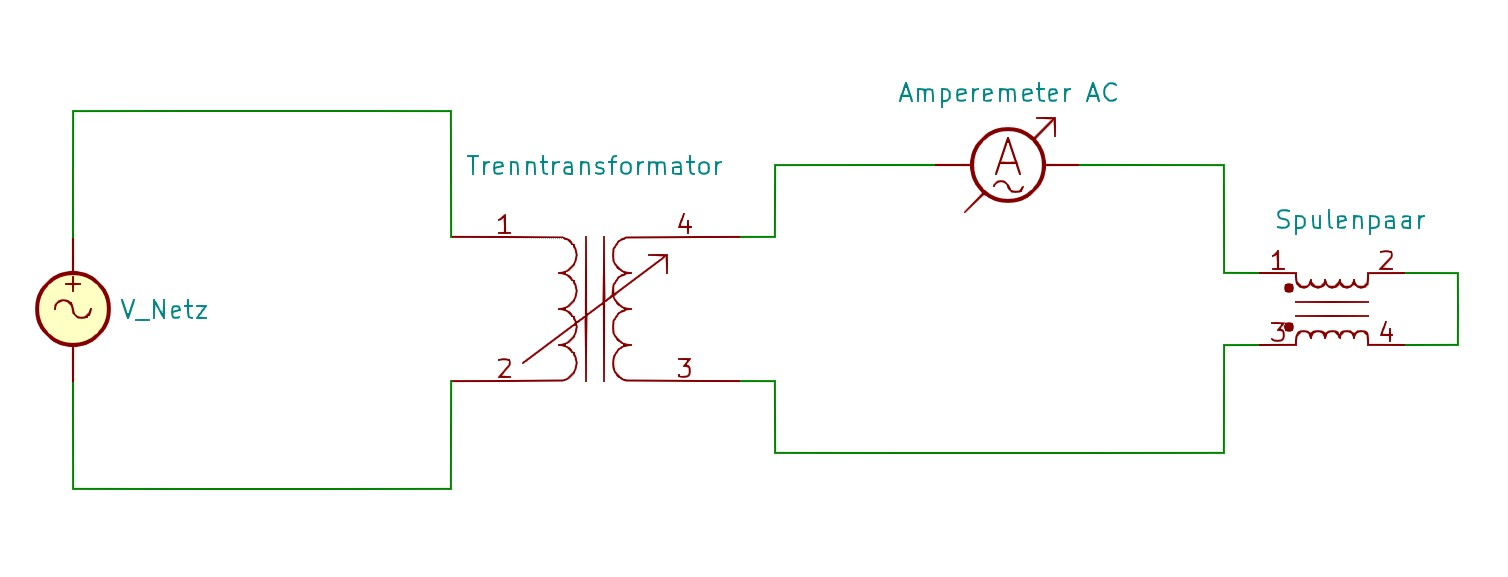
\includegraphics[width=.8\textwidth]{kicad/abbildungen/schematic_entmagnetisierung.jpg}
    \caption[Schaltskizze zur Entmagnetisierung]{Elektrischer Aufbau zur Entmagnetisierung der Spulen und des Eisenkerns.}%
    \label{fig:schematicEntmag}
\end{figure}

\begin{figure}[h]
    \centering
    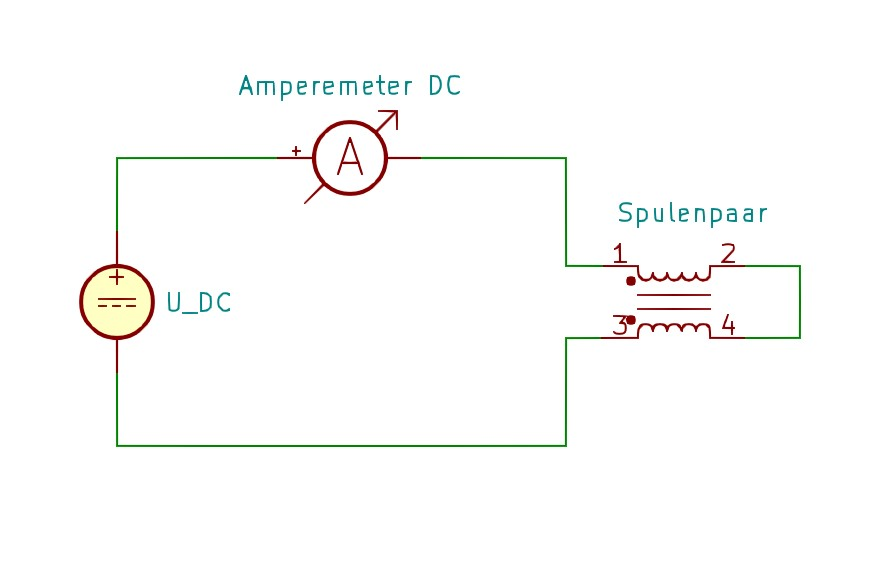
\includegraphics[width=.8\textwidth]{kicad/abbildungen/schematic_messung.jpg}
    \caption[Schaltskizze des Messaufbaus]{Elektrischer Aufbau zur Messung des Einflusses verschiedener Flussdichten auf die \textsc{Hall}-Spannung \(U_H\).}%
    \label{fig:schematicMessung}
\end{figure}


\begin{figure}[h]
    \centering
    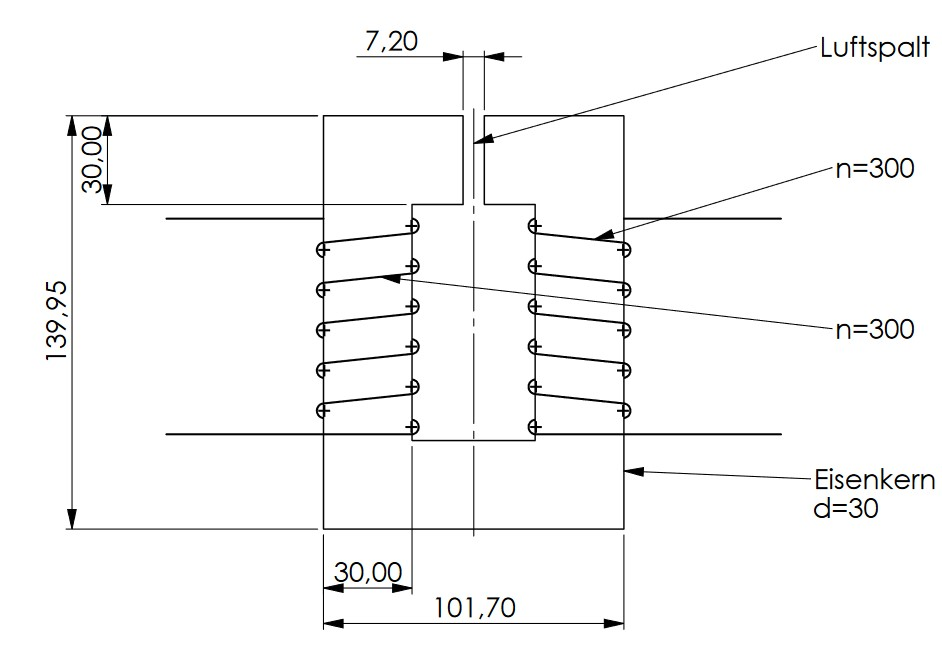
\includegraphics[width=.8\textwidth]{CAD/kern.jpg}
    \caption[Skizze des Spulenpaares mit Eiskenkern und Luftspalt]{Aufbau und Dimensionen des Eisenkerns mit Luftspalt und des Spulenpaares. Längeneinheiten in \si{\milli\metre}.}%
    \label{fig:zeichnungKern}
\end{figure}
\input{chapters/4_durchführung}
\chapter{Auswertung}
\section{Flussdichte}
Die mittlere Strecke entlang des Eisenkerns beträgt
\begin{equation}
    \bar{s_{Fe}} = 2 \cdot (\SI{139,95}{mm} + \SI{101,7}{mm} + 2 \cdot \SI{30}{mm}) - \SI{7,2}{mm} = \SI{596,1}{mm}
\end{equation}
Die des Luftspaltes ist trivial und beträgt \(s_L=\SI{7,2}{mm}\) (vgl. \cref{fig:zeichnungKern}).
\par\medskip
Der sich für einen Spulenstrom von \SI{2,4}{A} einstellende Fluss berechnet sich mit Hilfe der Gleichungen \cref{eq:NI}
bis \cref{eq:Rm} zu
\begin{gather}
    N \cdot I_S = \Phi \cdot \left(\frac{\bar{s_{Fe}}}{\mu_o\mu_{r,Fe}A} + \frac{s_L}{\mu_0 A}\right) \nonumber \\
    \Leftrightarrow \nonumber \\
    \Phi = N \cdot I_S \cdot A \cdot \mu_0 \cdot \left(\frac{\bar{s_{Fe}}}{\mu_{r,Fe}} + s_L\right)^{-1}
    \label{eq:fluss}
\end{gather}
Durchdringt der magnetische Fluss eine ebene Fläche entlang ihrer Normalen ist die Flussdichte dargestellt durch
\begin{equation}
    B = \frac{\Phi}{A}
    \label{eq:flussdichte}
\end{equation}
Im vorliegenden Fall ist die Fläche über die gesamte Strecke konstant. \cref{eq:flussdichte} in \cref{eq:fluss} eingesetzt
verschwindet die Fläche. Mit den Werten \(\mu_{r,Fe}=500\), \(\bar{s_{Fe}}=\SI{596,1}{mm}\), \(s_L=\SI{7,2}{mm}\), \(n=300\),
\(I_S=\SI{2,4}{A}\) und um den Faktor \(2\) multipliziert ergibt sich so eine rechnerische Flussdichte von
\begin{align}
    B &= 2 \cdot \frac{n \cdot I_S \cdot \mu_0}{\left( \frac{\bar{S_{Fe}}}{\mu_{r,Fe}}\right) + s_L} \nonumber \\
    &= 2\cdot \frac{300 \cdot \SI{2,4}{A} \cdot 4\pi \cdot \SI{10^{-7}}{\volt\second\per\ampere\per\metre}}{ \left( \frac{\SI{0,5961}{m}}{500} \right) + \SI{0,0072}{m} } \nonumber \\
    &\approx \SI{215,624}{mT}
\end{align}
Der Faktor \(2\) trägt der Tatsache Rechnung, dass im vorliegenden Aufbau zwei Spulen mitläufig angeordnet und verschaltet
sind.
\par
Der rechnerische Wert für die Flussdichte weicht um etwa \SI{32}{mT} vom messtechnisch ermittelten Wert ab. Die Differenz
lässt sich durch Vereinfachungen der Gleichung, so wie durch Toleranzen im Messaufbau erklären.
%
%==================================================================
%
\section{Probenparameter}
\begin{figure}[H]
    \centering
    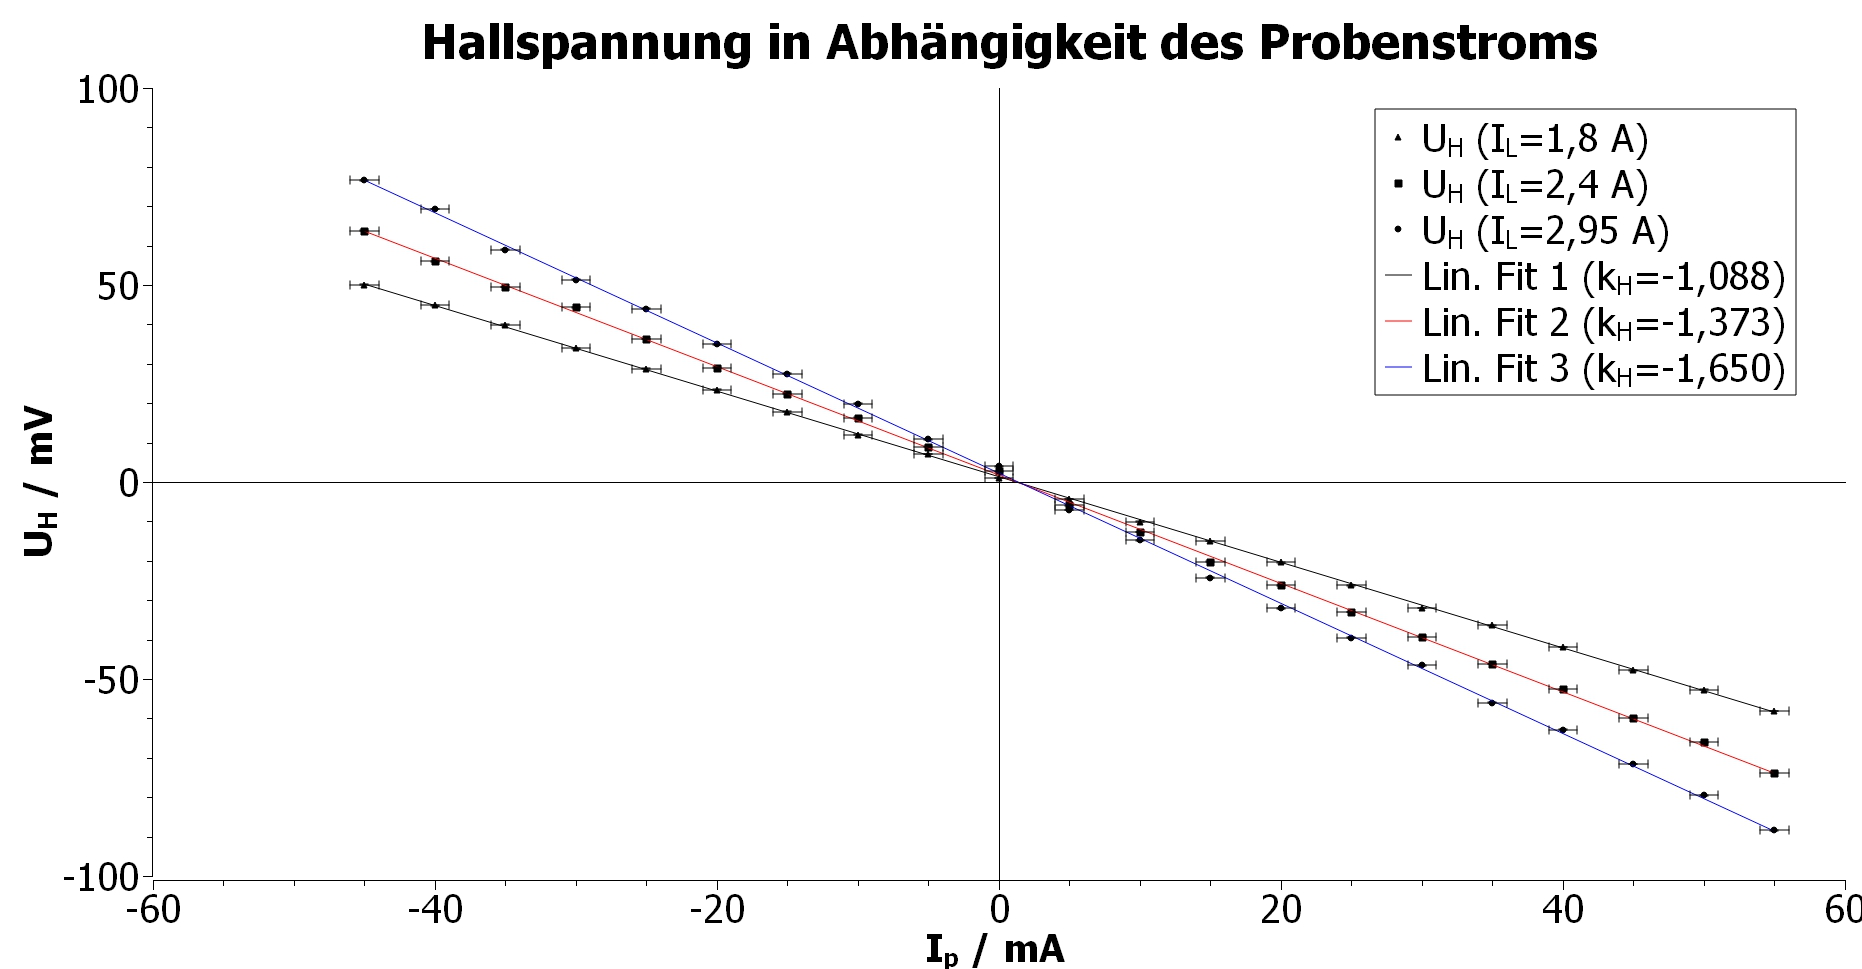
\includegraphics[width=\textwidth]{scidavis/abbildungen/hallspannung.jpeg}
    \caption[Diagram der Messwerte $U_H(I_p)$]{Gemessene Hallspannung $U_H$ aufgetragen über den Probenstrom $I_p$ für drei verschiedene Spulenspannungen $I_L$.}%
    \label{fig:hallspannung}
\end{figure}

Der \textsc{Hall}-Koeffizient ist mit \(A_H = (qn_q)^{-1}\) ein materialabhängiger Parameter und dient als Proportionalitätsfaktor der \textsc{Hall}-Spannung \(U_H\).
Aus \cref{eq:UH2} lässt er sich bestimmen durch
\begin{equation}
   A_H = \frac{U_H \cdot b}{B \cdot I_p} = \frac{k_H \cdot b}{B} = \frac{1}{q \cdot n_q}%
   \label{eq:hallKoeff}
\end{equation}
\(k_i\) sind hier die Steigungen des \(U_H(I_p)\)-Diagramms mit den zugehörigen Flussdichten \(B_i\).
Daraus ergibt sich ein mittlerer wert für den \textsc{Hall}-Koeffizienten zu
\begin{equation}
    A_H = \frac{\SI{-1,373}{\volt\per\ampere} \cdot \SI{0,001}{m}}{\SI{0,248}{T}}
    \approx \SI{-5,5 \cdot 10^{-3}}{\metre\cubed\per\ampere\per\second}
\end{equation}
mit einer Unsicherheit von
\begin{align}
    \Delta A_H &= \left| \partial A_H \over \partial k_H \right| \cdot \Delta k_H + \left| \partial A_H \over \partial h \right| \cdot \Delta h + \left| \partial A_H \over \partial B \right| \cdot \Delta B \nonumber \\
    &= \left| \frac{h}{B} \right| \cdot \Delta k_H + \left| \frac{k_H}{B} \right| \cdot \Delta h + \left| \frac{k_H \cdot h}{B^2} \right| \cdot \Delta B \nonumber \\
    &= 
    \frac{\SI{0,01}{m}}{\SI{0,248}{T}} \cdot \SI{0,0049}{\volt\per\ampere} + 
    \frac{\SI{1,373}{\volt\per\ampere}}{\SI{0,248}{T}} \cdot \SI{10^{-4}}{m} + 
    \frac{\SI{1,373}{\volt\per\ampere} \cdot \SI{10^{-3}}{m}}{\SI{0,248^2}{T^2}} \cdot \SI{10^{-4}}{T} \nonumber \\
    &= \pm \SI{0,8 \cdot 10^{-3}}{\metre\cubed\per\ampere\per\second}
\end{align}
\par\medskip
Die Ladungsträgerkonzentration \(n_q\) lässt sich analog dazu berechnen durch
\begin{align}
    n_q &= \frac{B}{k_H \cdot q \cdot b} \nonumber \\
    &= -\frac{\SI{0,248}{T}}{\SI{1,602}{As} \cdot \SI{0,001}{m} \cdot \SI{1,373}{\volt\per\ampere}} \cdot 10^{19} \nonumber \\
    &\approx \SI{1,128 \cdot 10^{21}}{m^{-3}}
\end{align}
Der Fehler beträgt hier
\begin{align}
    \Delta n_q &=
    \left| \frac{\partial n_q}{\partial b} \right| \cdot \Delta b +
    \left| \frac{\partial n_q}{\partial B} \right| \cdot \Delta B +
    \left| \frac{\partial n_q}{\partial k_H} \right| \cdot \Delta k_H \nonumber \\
    &= \left| \frac{B}{k_H \cdot q \cdot b^2} \right| \cdot \Delta b +
    \left| \frac{1}{k_H \cdot q \cdot b} \right| \cdot \Delta B +
    \left| \frac{B}{k_H^2 \cdot q \cdot b} \right| \cdot \Delta k_H \nonumber \\
    &= \frac{10^{19}}{\SI{1,602}{As}} \cdot \Bigg[\left( \frac{\SI{0,248}{T}}{\SI{1,373}{\volt\per\ampere} \cdot \SI{10^{-6}}{m^2}} \right) \cdot \SI{10^{-4}}{m}
    + \left( \frac{1}{\SI{1,373}{\volt\per\ampere} \cdot \SI{10^{-3}}{m}} \right) \cdot \SI{10^{-4}}{T} \nonumber \\
    &\quad + \left( \frac{\SI{0,248}{T}}{ \left( \SI{1,373}{\volt\per\ampere} \right)^2 \cdot \SI{10^{-3}}{m}} \right) \cdot 4,9 \cdot \SI{10^{-3}}{\volt\per\ampere} \Bigg] \nonumber \\
    &= \pm 1,173 \cdot \SI{10^{20}}{m^{-3}}
\end{align}

\par\medskip
%
%===================================================================
%
\begin{figure}[H]
    \centering
    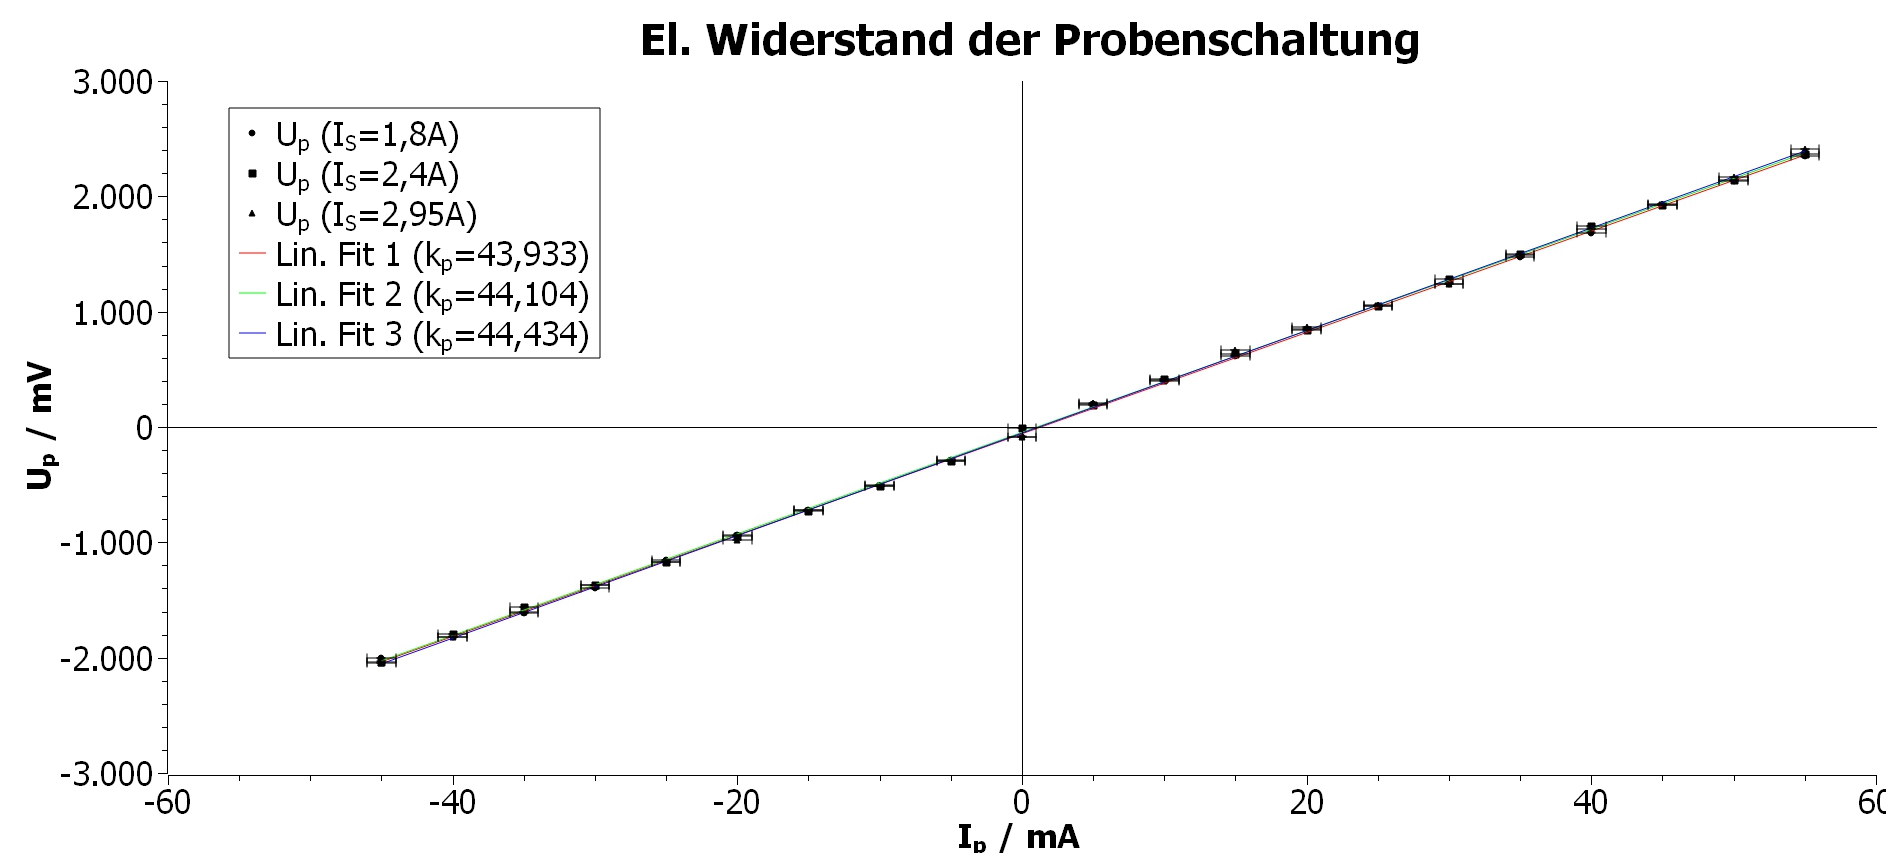
\includegraphics[width=\textwidth]{scidavis/abbildungen/R_probe.jpeg}
    \caption[Diagram der Messwerte \(U_p(I_p)\)]{Diagram der Messwerte \(U_p(I_p)\). Die Steigung des Linearen Fits \(k_p\) entspricht dem elektrischen Widerstand der Probenschaltung.}%
    \label{fig:Rprobe}
\end{figure}
Die Steigung des linearen Fits in \cref{fig:Rprobe} ist direkt als elektrischen Widerstand der Probe zu interpretieren.
Mit \cref{eq:spezR} lässt sich daraus der spezifische Widerstand \(\rho\)
\begin{equation}
    \rho = k_p \cdot \frac{b h}{l} = \SI{44,104}{\Omega} \cdot \frac{\SI{0,001}{m} \cdot \SI{0,01}{m}}{\SI{0,02}{m}} \approx \SI{0,022}{\Omega m}%
    \label{eq:spezRnum}
\end{equation}
und die Ladungsträgerbeweglichkeit \(\mu\) (nicht zu verwechseln mit der magnetischen Permeabilität) - ein Maß für
Driftgeschwindigkeit der Ladungsträger innerhalb eines elektrischen Feldes - innerhalb des Probenmaterials ermitteln.
\begin{equation}
    \mu = \frac{1}{\rho} \cdot A_H
    = \frac{1}{\SI{0,022}{\Omega m}}\cdot -\SI{5,54 \cdot 10^{-3}}{\metre\cubed\per\ampere\per\second}
    \approx -\SI{0,252}{\metre\squared\per\volt\second}
\end{equation}
%
\par
Die Fehler liegen hier bei
\begin{align}
    \Delta \rho &= \left| \frac{\partial \rho}{\partial k_p} \right| \cdot \Delta k_p +
    \left| \frac{\partial \rho}{\partial b} \right| \cdot \Delta b +
    \left| \frac{\partial \rho}{\partial h} \right| \cdot \Delta h +
    \left| \frac{\partial \rho}{\partial l} \right| \cdot \Delta l \nonumber \\
    &= \left| \frac{b \cdot h}{l} \right| \cdot \Delta k_p +
    \left| \frac{k_p \cdot h}{l} \right| \cdot \Delta b +
    \left| \frac{k_p \cdot b}{l} \right| \cdot \Delta h +
    \left| \frac{k_p \cdot b \cdot h}{l^2} \right| \cdot \Delta l \nonumber \\
    &= \left( \frac{\SI{10^{-3}}{m} \cdot \SI{10^{-2}}{m}}{2 \cdot \SI{10^{-2}}{m}} \right) \cdot \SI{0,136}{\volt\per\ampere} +
    \left( \frac{\SI{44,104}{\volt\per\ampere} \cdot \SI{10^{-2}}{m}}{2 \cdot \SI{10^{-2}}{m}} \right) \cdot \SI{10^{-4}}{m} \nonumber \\
    &\quad+ \left( \frac{\SI{44,104}{\volt\per\ampere} \cdot \SI{10^{-3}}{m}}{2 \cdot \SI{10^{-2}}{m}} \right) \cdot \SI{10^{-4}}{m} +
    \left( \frac{\SI{44,104}{\volt\per\ampere} \cdot \SI{10^{-3}}{m} \cdot \SI{10^{-2}}{m}}{4 \cdot \SI{10^{-4}}{m^2}} \right) \cdot \SI{10^{-4}}{m}\nonumber \\
    &= \pm 3 \cdot \SI{10^{-3}}{\Omega m}
\end{align}
und
\begin{align}
    \Delta \mu &=
    \left| \frac{\partial \mu}{\partial \rho} \right| \cdot \Delta \rho +
    \left| \frac{\partial \mu}{\partial A_H} \right| \cdot \Delta A_H \nonumber \\
    &=
    \left| \frac{A_H}{\rho^2} \right| \cdot \Delta \rho +
    \left| \rho^{-1} \right| \cdot \Delta A_H \nonumber \\
    &=
    \left( \frac{5,54 \cdot \SI{10^{-3}}{\metre\cubed\per\ampere\per\second}}{\left( \SI{0,022}{\Omega m} \right)^2} \right) \cdot 3 \cdot \SI{10^{-3}}{\Omega m} +
    \left( \SI{0,022}{\Omega m} \right)^{-1} \cdot 7,534 \cdot \SI{10^{-4}}{\Omega} \nonumber \\
    &= \pm \SI{0,069}{\metre\squared\per\volt\second}
\end{align}
\section{Messunsicherheiten}
\begin{table}[h]
    \centering
    \begin{tabular}{@{}ll@{}}
        \toprule
        Größe                                            & Wert                                                                    \\ \midrule
        \textsc{Hall}-Koeffizient $A_H$                  & \( (-5,54 \cdot 10^{-3} \pm 7,534 \cdot 10^{-4})\SI{}{\Omega}\)         \\
        Ladungsträgerdichte $n_q$                        & \( (1,128 \cdot 10^{21} \pm 1,173 \cdot 10^{20})\SI{}{m^{-3}}\)         \\
        Spezifischer Widerstand \(\rho\)                 & \( (0,022 \pm 3 \cdot 10^{-3})\SI{}{\Omega m} \)                        \\
        Ladungsträgerbeweglichkeit \(\mu\)               & \( (-0,252 \pm 0,069)\SI{}{\metre\squared\per\volt\second} \)                           \\ \bottomrule
    \end{tabular}
\end{table}
\chapter{Fazit}
Bei einem Probenstrom von \SI{0}{A} ist nach \cref{eq:UH2} eine \textsc{Hall}-Spannung von \SI{0}{V} zu erwarten. Der Offset
der \textsc{Hall}-Spannung in \cref{fig:hallspannung} lässt auf eine unsaubere Fehlspannungskorrektur schließen. Da in Folgenden
Berechnungen allerdings die Steigung eingeht und diese unempfindlich gegenüber Verschiebungen entlang der \(x\)- und \(y\)-Achse
ist, wird angenommen, dass dieser Offset eine untergeordnete Rolle spielt. Interessanter ist jedoch, dass obschon eine
Fehlspannungskorrektur gemäß Versuchsanleitung mit bei einem Probenstrom von \SI{5}{mA} durchgeführt wurde, sich die
\(x\)-Achsenabschnitte der linearen Fits aller drei Messreihen bei \(\approx \SI{2,5}{mA}\) wiederfinden. Das spricht für
einen gegenüber dem angenommenen Messfehler für \(\Delta I_p = \SI{1}{mA}\) nicht zu ignorierend höheren Messfehler von
\(250\%\). Selbiges spiegelt sich auch \cref{fig:Rprobe} wieder.
\par\medskip
Es wurde während der Messung versäumt die Dimensionen und weitere Spezifikationen der Probe aufzuzeichnen. Für die Auswertung
wurden Werte für \(l\text{, }b\text{und }h\) dem Datenblatt des Herstellers \autocite{PHYWESystemeGmbHundCo.KG.} entnommen.
Da aus diesem allerdings keine Messunsicherheiten hervorgehen wurden für die drei Längenangaben jeweils \(\pm\SI{0,1}{mm}\)
angenommen.
\par
Ebenfalls wurde vom Experimentator die Temperaturabhängigkeit der Ladungsträgerbeweglichkeit und -konzentration nicht in
Betracht gezogen. Durch \cref{eq:hallKoeff} hängt hiermit direkt der \textsc{Hall}-Koeffizient und damit die Höhe der \textsc{Hall}-Spannung
zusammen. Da der Probenstrom am Innenwiderstand der Probe eine Verlustleistung erzeugt und die Probe damit erwärmt, ist
mit fortschreitenden Messungen eine Verzerrung der \textsc{Hall}-Spannung zu rechnen.
\par\medskip
Mit einem negativen Vorzeichen des \textsc{Hall}-Koeffizienten und der hierdurch ebenfalls negativen Ladungsträgerbeweglichkeit
\(\mu\) ist anzunehmen, dass es sich bei der Probe um p-dotiertes Germanium handelt. Hier bilden \textit{Löcher} als positive
pseudo-Ladungsträger den Stromfluss. Entsprechend fließen innerhalb des Germaniumkristalls freie Elektronen in entgegen gesetzter
Richtung. Diese sind es jedoch, die unter Einfluss eines äußeren magnetischen Feldes der \textsc{Lorentz}-Kraft unterliegen
und in ihrer Bahn so abgelenkt werden, dass sich die \textsc{Hall}-Spannung wie eingangs beschrieben ausbilden kann. Siehe auch
\cref{eq:UH1}: eine Umkehr der Ausrichtung der Driftgeschwindigkeit \(\vec{v_D}\) geht mit einer Vorzeichenumkehr der Hallspannung
einher.
\par\medskip
Im allgemeinen liegen die Messunsicherheiten bei \(\approx 13-14\%\) während der für die Ladungsträgerbeweglichkeit bei
nahe \(30\%\) liegt. Über Lehr- und Demonstrationszwecke hinaus ist der Aufbau - subjektiv - als ungeeignet einzuordnen.
\par\bigskip
Zuletzt ist anzumerken, dass die Versuchsanleitung zu wünschen übrig lässt. Falsche Schaltbilder, irreführende Beschreibungen
und ausgelassene wichtige Hinweise haben sowohl den initialen Aufbau, wie auch die Durchführung und Auswertung erheblich
erschwert. Die Kürze der Bearbeitungszeit außer Acht gelassen hat dies jedoch zu einer tiefergehenden Auseinandersetzung
mit der Thematik angeregt.
%-------------------
\newpage
\listoffigures 
\listoftables
\addchap{Verwendete Symbole}

\begin{table}[h]
    \begin{tabular}{@{}ll@{}}
        $A$ & Fläche \\
        $A_H$ & \textsc{Hall}-Koeffizient\\
        $\vec{B}$           & Magnetisches Feld \\
        $\vec{F_E}$           & Elektrische Feldkraft \\
        $\vec{F_L}$           & Lorentzkraft \\
        $\vec{H}$ & Magnetische Feldstärke \\
        $R$ & Elektrischer Widerstand \\
        $R_m$ & Magnetischer Widerstand \\
        $I_p$  & Probenstrom \\
        $I_S$  & Spulenstrom \\
        $N$ & Windungszahl \\
        $U_H$  & \textsc{Hall}-Spannung \\
        $U_p$  & Spannungsabfall an der Probe \\
        & \\
        $b$           & Breite der Probe \\
        $h$           & Höhe der Probe \\
        $j$ & Stromdichte \\
        $k_H$ & Steigung im \(U_H(I_p)\)-Diagram \\
        $k_p$ & Steigung im \(U_p(I_p)\)-Diagram \\
        $l$           & Länge der Probe \\
        $n_q$ & Ladungsträgerdichte \\
        $q$           & Ladung \\
        $\bar{s_{Fe}}$ & Mittlere Länge des Eisenkerns \\
        $s_L$ & Länge des Luftspalts \\
        $\vec{v_D}$           & Driftgeschwindigkeit \\
        & \\
        $\Phi$ & Magnetischer Fluss \\
        $\Theta$ & Magnetische Durchflutung \\
        $\mu$ & Ladungsträgerbeweglichkeit \\
        $\mu_0$ & Permeabilität des Vakuums \\
        $\mu_r$ & Relative Permeabilität \\
        $\rho$ & Spezifischer elektrischer Widerstand \\
    \end{tabular}
\end{table}
\appendix
\chapter{Anhang}
\begin{table}[h]
    \centering
    \caption[Messtechnisch ermittelte Flussdichten]{Im Luftspalt gemessene Flussdichten $B$ bei verschiedenen Spulenströmen.}
    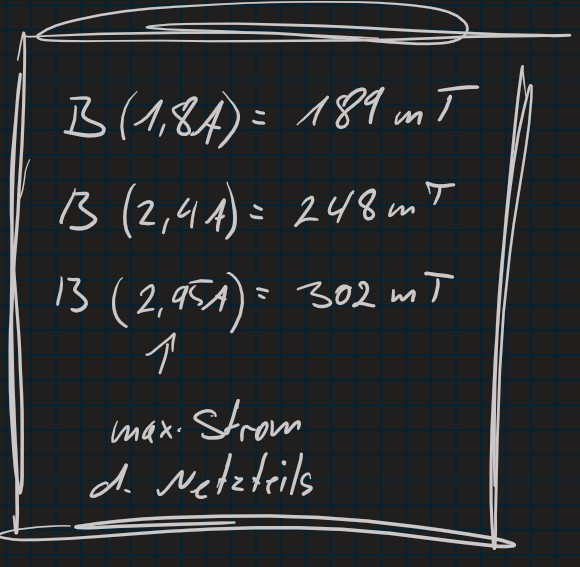
\includegraphics[height=.5\textheight]{messungen/messungen_flussdichte.jpg}
    \label{tab:messwerte_flussdichte}
\end{table}

\begin{table}[h]
    \centering
    \caption[Messwertetabelle]{Messwerte für \textsc{Hall}-Spannungen $U_H$ und Probenspannungen $U_p$ bei verschiedenen Probenströmen $I_p$ mit dem Spulenstrom $I_S$ als Parameter.}
    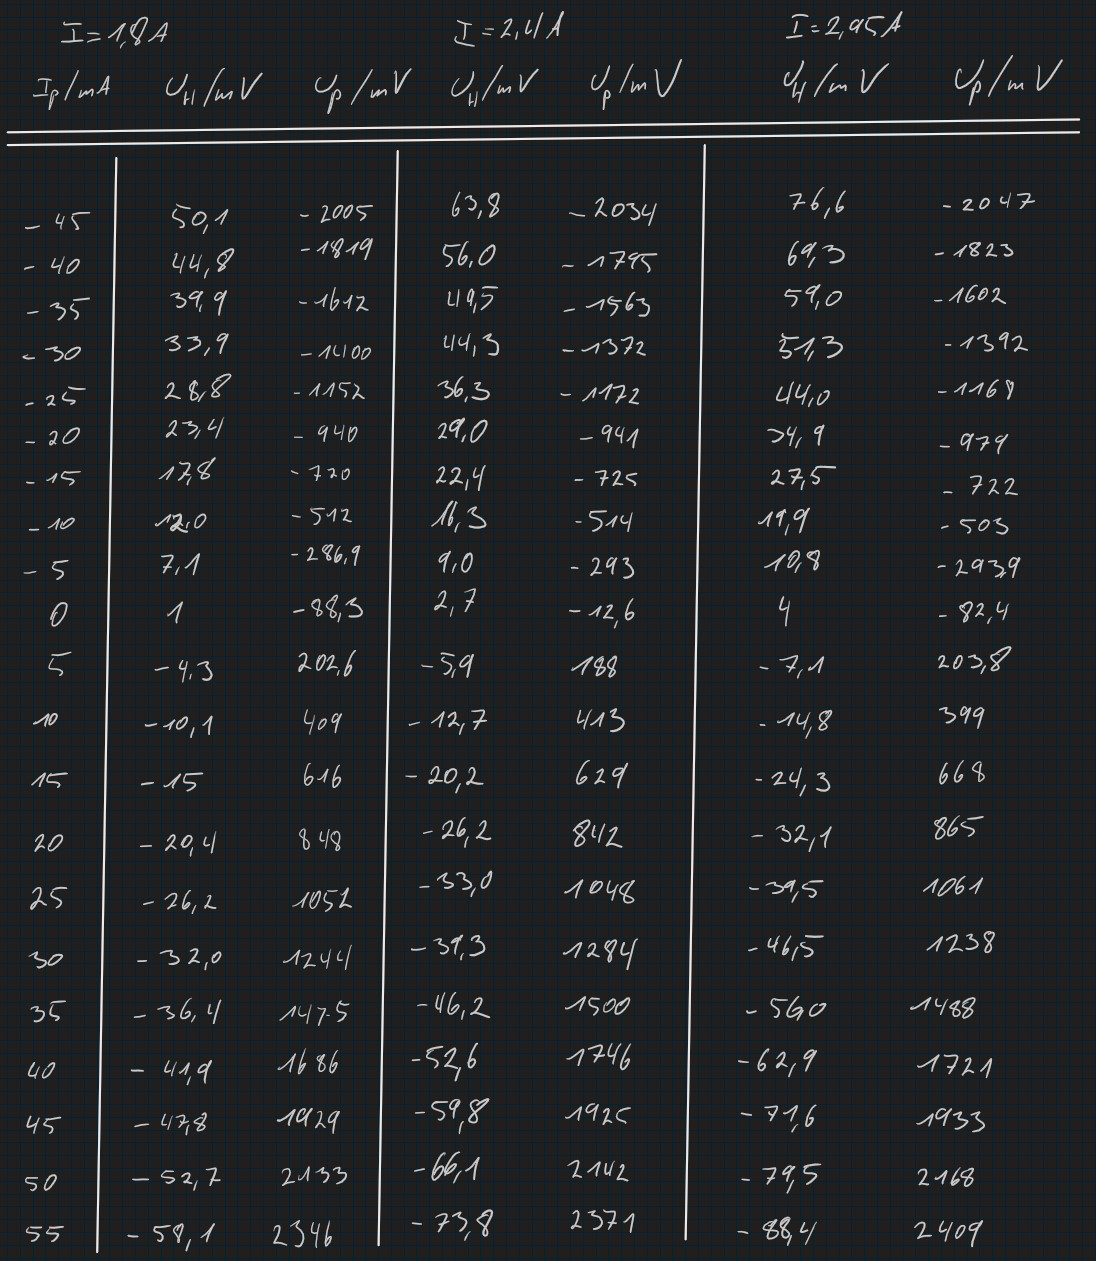
\includegraphics[height=.8\textheight]{messungen/messungen.jpg}
    \label{tab:messwerte}
\end{table}
\printbibliography%
%\bibliographystyle{plaindin}
%==========================================
\end{document}